% Presentation on Face Detection
% Evangelos Foutras <foutrelis@gmail.com>
% University of Piraeus
% May 27th 2009

% TODO: Reference other presentations from which images were taken

\documentclass{beamer}

\usepackage{xunicode}
\usepackage{xltxtra}
\usepackage{xgreek}
\usepackage{graphics}
\usepackage{ulem}
\setsansfont[Mapping=tex-text]{Verdana}

\usetheme{Warsaw}
\setbeamertemplate{navigation symbols}{}

\title[Ανίχνευση προσώπων με Haar-like χαρακτηριστικά]{Ανίχνευση προσώπων\\με χρήση χαρακτηριστικών
	τύπου Haar}
\author{Ευάγγελος Φούτρας -- Π/06156}
\institute{Πανεπιστήμιο Πειραιώς}
\date{27 Μαΐου 2009}
\usepackage{graphicx}

\begin{document}

\begin{frame}
\titlepage
\end{frame}

\begin{frame}
\frametitle{Επισκόπηση}
\begin{itemize}
\item Προτάθηκε από τους Paul Viola και Michael Jones
\item Επεκτάθηκε από τον Rainer Lienhart
\item Χαρακτηριστικά τύπου Haar (Haar-like features)
\item Πίνακας Προστιθέμενου Εμβαδού
\item Αλγόριθμος ενδυνάμωσης AdaBoost
\item Διαδοχικά συνδεδεμένοι ταξινομητές (cascade)
\end{itemize}
\end{frame}

\begin{frame}
\frametitle{Haar-like χαρακτηριστικά}
\begin{itemize}
\item Χαρακτηριστικά δύο, τριών και τεσσάρων ορθογωνίων
\item Οι λευκές περιοχές αφαιρούνται από τις μαύρες
\item Υπολογίζονται πολύ γρήγορα\\
	(με \textbf{Πίνακα Προστιθέμενου Εμβαδού})
\end{itemize}

\begin{center}
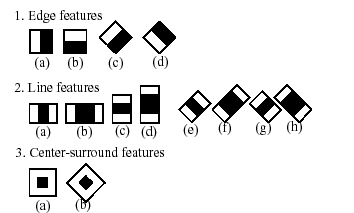
\includegraphics[width=0.6\textwidth]{images/feature-types}
\end{center}
\end{frame}

\begin{frame}
\frametitle{Πίνακας Προστιθέμενου Εμβαδού}
Μπορεί να υπολογιστεί με ένα μόνο πέρασμα της εικόνας:
\begin{equation*}
sat(x,y) = i(x,y) + sat(x-1,y) + sat(x,y-1) - sat(x-1,y-1)
\end{equation*}

\begin{center}
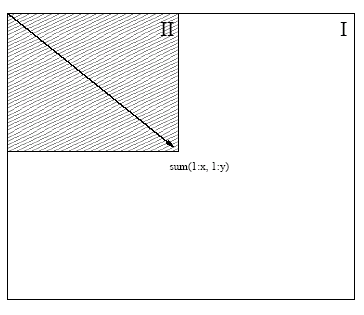
\includegraphics[width=0.5\textwidth]{images/integral-image-generation}
\end{center}
\end{frame}

\begin{frame}
\frametitle{Υπολογισμός εμβαδού}
\begin{center}
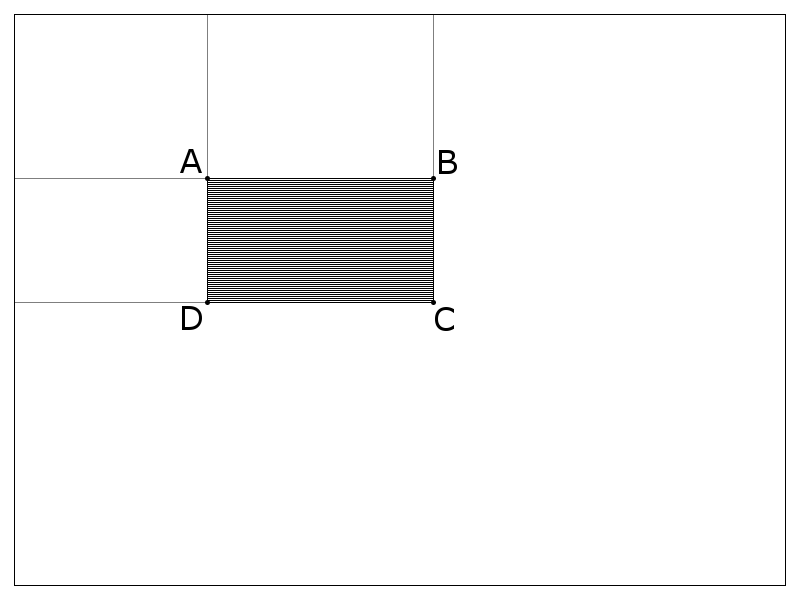
\includegraphics[width=0.7\textwidth]{images/integral-image}
\begin{equation*}
sum = sat(A) + sat(C) - sat(B) - sat(D)
\end{equation*}
\end{center}
\end{frame}

\begin{frame}
\frametitle{Εξαγωγή χαρακτηριστικών}
\begin{itemize}
\item Υπο-παράθυρα των 20x20 εικονοστοιχείων
\item Όλες οι δυνατές θέσεις και διαστάσεις κάθε τύπου
\item Αρκετές δεκάδες χιλιάδες χαρακτηριστικά σύνολο (> 100.000)
\end{itemize}
\begin{center}
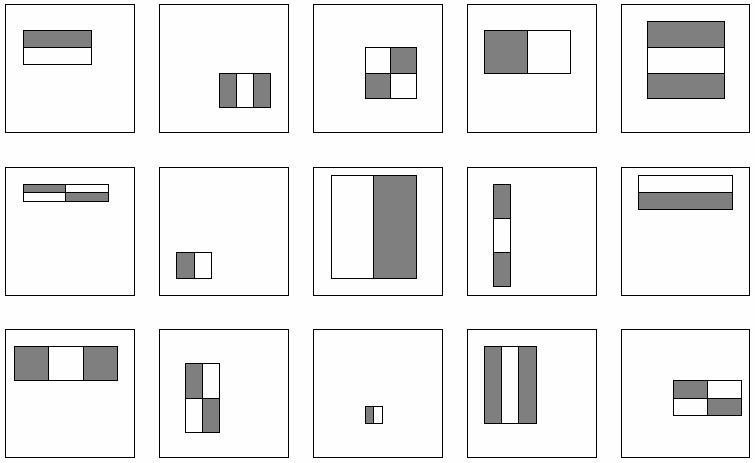
\includegraphics[width=0.7\textwidth]{images/features-in-subwindows}
\end{center}
\end{frame}

\begin{frame}
\frametitle{Ασθενής αλγόριθμος ταξινόμησης}
\begin{itemize}
\item Για κάθε χαρακτηριστικό τύπου Haar, ορίζεται μία ασθενής συνάρτηση
ταξινόμησης $h_j$ ως εξής:

\begin{equation*}
h_j(x) = \begin{cases}
	1, & \mbox{εάν } p_jf_j(x) < p_j\theta_j \\
	0, & \mbox{αλλιώς}
\end{cases}
\end{equation*}
όπου το $x$ είναι ένα υπο-παράθυρο, το $\theta$ ένα κατώφλι και το $p_j$
υποδηλώνει τη φορά της ανίσωσης.
\end{itemize}
\end{frame}

\begin{frame}
\frametitle{Αλγόριθμος ενδυνάμωσης Adaboost}
\begin{itemize}
\item Επιλεκτικός συνδυασμός ασθενών ταξινομητών
\begin{itemize}
\item Αρχικά όλα τα παραδείγματα έχουν το ίδιο βάρος
\item Σε κάθε επανάληψη υπολογίζεται η τιμή των ασθενών συναρτήσεων για κάθε
παράδειγμα
\item Για κάθε συνάρτηση επιλέγεται το καλύτερο κατώφλι
\item Επιλέγεται ο ασθενής ταξινομητής με το μικρότερο ποσοστό λάθους
\item Αυξάνεται το βάρος των παραδειγμάτων που δεν ταξινομήθηκαν σωστά
\end{itemize}
\item Το αποτέλεσμα είναι ένας ισχυρός ταξινομητής
\end{itemize}
\end{frame}

\begin{frame}
\frametitle{Παράδειγμα ενδυνάμωσης AdaBoost}
\begin{center}
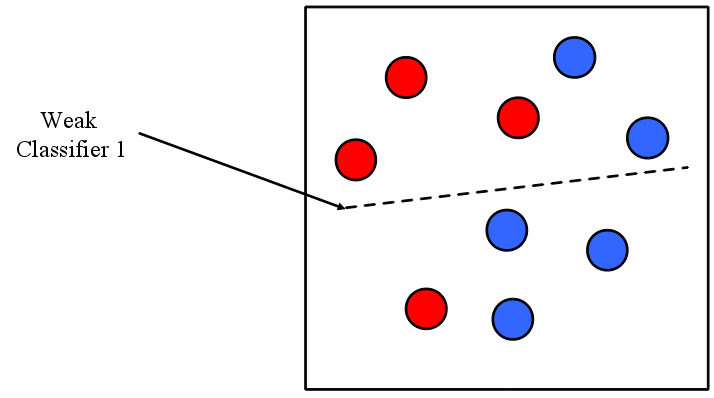
\includegraphics[width=0.8\textwidth]{images/boosting/boosting-1}
\end{center}
\end{frame}

\begin{frame}
\frametitle{Παράδειγμα ενδυνάμωσης AdaBoost}
\begin{center}
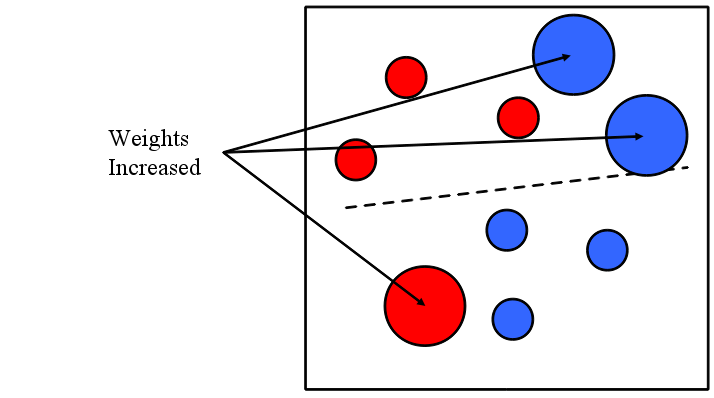
\includegraphics[width=0.8\textwidth]{images/boosting/boosting-2}
\end{center}
\end{frame}

\begin{frame}
\frametitle{Παράδειγμα ενδυνάμωσης AdaBoost}
\begin{center}
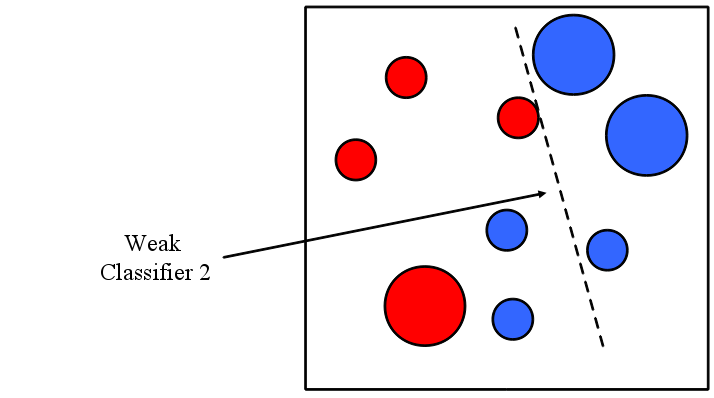
\includegraphics[width=0.8\textwidth]{images/boosting/boosting-3}
\end{center}
\end{frame}

\begin{frame}
\frametitle{Παράδειγμα ενδυνάμωσης AdaBoost}
\begin{center}
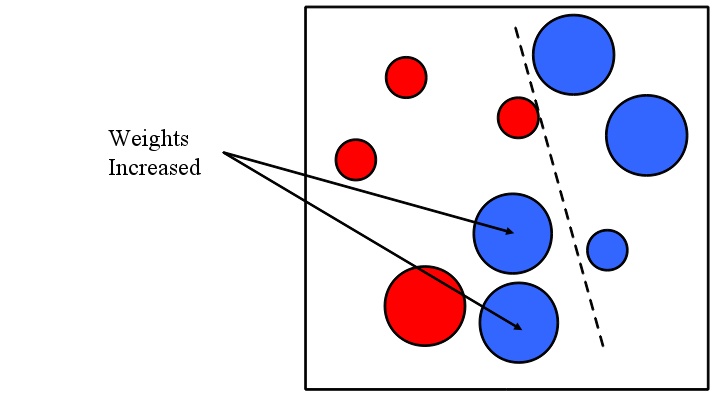
\includegraphics[width=0.8\textwidth]{images/boosting/boosting-4}
\end{center}
\end{frame}

\begin{frame}
\frametitle{Παράδειγμα ενδυνάμωσης AdaBoost}
\begin{center}
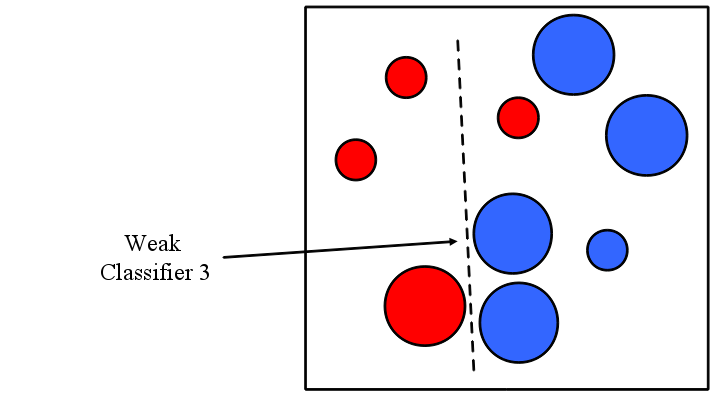
\includegraphics[width=0.8\textwidth]{images/boosting/boosting-5}
\end{center}
\end{frame}

\begin{frame}
\frametitle{Παράδειγμα ενδυνάμωσης AdaBoost}
\begin{center}
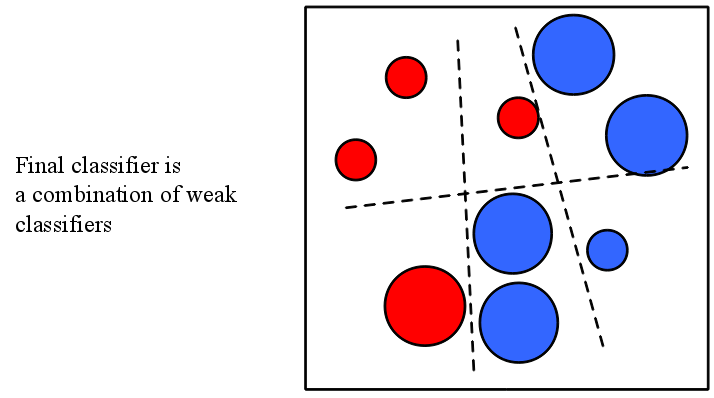
\includegraphics[width=0.8\textwidth]{images/boosting/boosting-6}
\end{center}
\end{frame}

\begin{frame}
\frametitle{Πρώτα χαρακτηριστικά που επιλέχθησαν}
Τα δύο πρώτα χαρακτηριστικά που επιλέχθησαν από τον αλγόριθμο ενδυνάμωσης:

\begin{center}
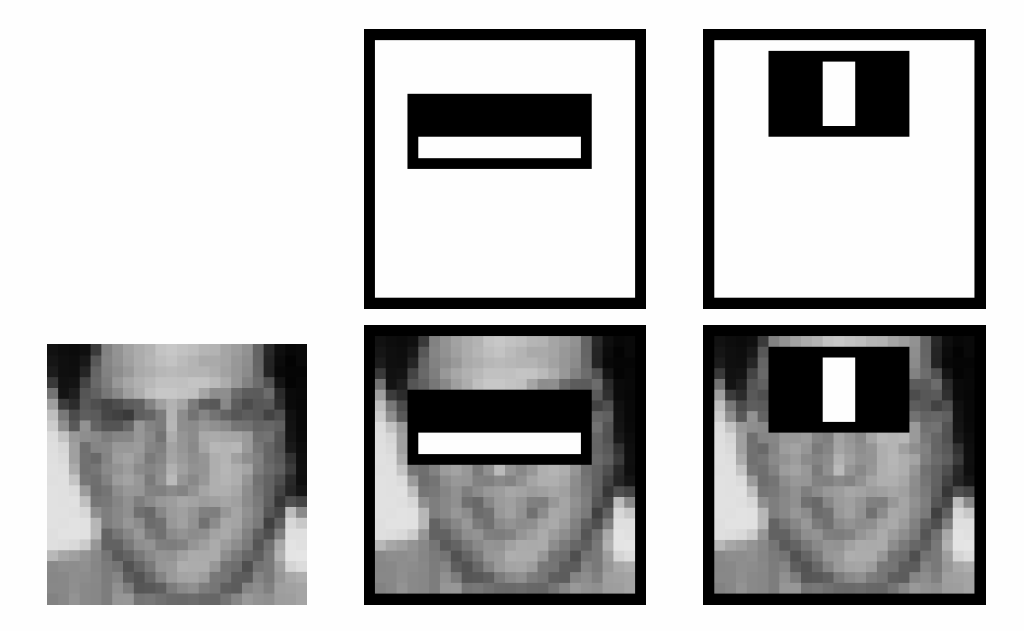
\includegraphics[width=0.5\textwidth]{images/feature-selection}
\end{center}

Ο παραπάνω συνδυασμός μπορεί να επιτύχει 100\% ποσοστό ανίχνευσης και 50\%
ποσοστό λανθασμένων ανιχνεύσεων.
\end{frame}

\begin{frame}
\frametitle{Διαδοχικά συνδεδεμένοι ταξινομητές}
\begin{itemize}
\item Κάθε υπο-παράθυρο περνάει από μία σειρά από ταξινομητές
\item Ο πρώτος ταξινομητής απορρίπτει πολλά από τα αρνητικά υπο-παράθυρα
\item Κάθε επόμενος ταξινομητής απορρίπτει επιπλέον αρνητικά υπο-παράθυρα, αλλά
απαιτεί περισσότερη υπολογιστική ισχύ
\end{itemize}

\begin{center}
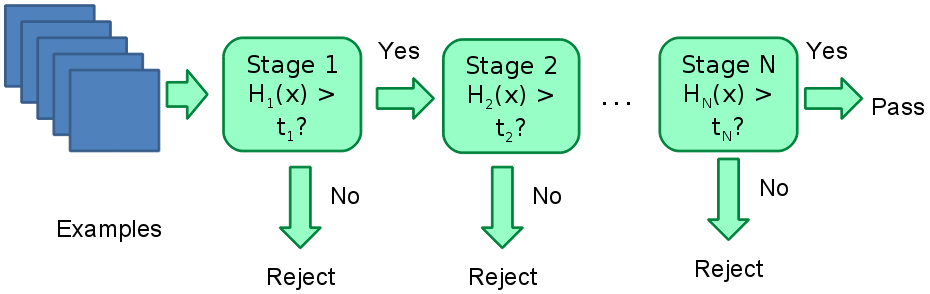
\includegraphics[width=0.8\textwidth]{images/cascade}
\end{center}
\end{frame}

\begin{frame}

\includegraphics[width=\textwidth]{images/not-finished}
\end{frame}

\begin{frame}
\frametitle{Παράδειγμα εφαρμογής}
\begin{itemize}
\item Ο κώδικας είναι διαθέσιμος στη διεύθυνση:
\textbf{http://github.com/foutrelis/facedet}
\item Χρησιμοποιεί τη βιβλιοθήκη ανοιχτού κώδικα \textbf{OpenCV} που υλοποιεί
	τον αλγόριθμο ανίχνευσης προσώπων που περιγράφηκε\\
	\textbf{http://opencv.willowgarage.com}
\end{itemize}
\end{frame}

\end{document}
